\section{Statik}

\begin{multicols}{2}
\textbf{Generelles Vorgehen} \\
1. Skizze mit allen Kräften aufzeichnen \\
2. Koordinatensystem einführen \\
3. Falls nötig, Drehpunkt von Drehmoment einführen \\
4. Gleichgewichtsbedingungs-/ Gleichungssystem aufstellen \\
5. Gleichungssystem auflösen \\
\columnbreak
\\
\textbf{Gleichgewichtsbedingung starrer Körper} \\
Ein Körper ist dann im Gleichgewicht, wenn keine resultierende Kraft auf ihn wirkt, d.h. die Summe der ihn angreifenden Kräfte ist null. \\
$\sum\limits_{i=0}^{n} F_{ix} = 0,  \; \sum\limits_{i=0}^{n} F_{iy} = 0, \; \sum\limits_{i=0}^{n} F_{iz} = 0 $
\end{multicols}

\subsection{Starrer Körper - Statik des Massenpunktes}
Ein Massenpunkt ist ein Körper, dessen ganze Masse in 
einem Punkt konzentriert ist. \\
Ein starrer Körper wird durch die an ihm angreifenden 
Kräfte nicht deformiert. Die Gerade, die durch den Angriffspunkt einer Kraft F geht und 
deren Richtung durch die Richtung von F bestimmt ist, wird 
Wirkungslinie von  F genannt. Für starre Körper gilt nun 
folgender Satz:
\textit{In einem starren Körper kann eine Kraft entlang ihrer 
Wirkungslinie beliebig verschoben werden, ohne dass sich 
an ihrer Wirkung etwas ändert.} 



\subsubsection{Kontaktkraft}
Bezeichnet die Kraft eines auf einer Oberfläche liegenden Körpers, die der Schwerkraft entgegenwirkt. Sie steht immer im rechten Winkel zur Ebene und zur Reibungskraft $F_R$. \\


\subsubsection{Reibung \& Gleitreibung}
\begin{minipage}{15.5cm}
Reibungskraft $F_{R} = \mu_{H} \cdot F_{N}$ (Der Körper haftet noch immer am Untergrund)\\
Gleitreibungskraft $F_G =  \mu_{G} \cdot F_{N}$ (Der Körper bewegt sich) \\
Achtung: Bei Schiefen Ebenen entspricht $F_{N}$ nicht $F_{G}$ \\
Die Reibungskraft ist nicht von der Grösse der Kontaktfläche abhängig, sondern nur vom Gewicht. \\
Die Reibungskraft geht immer in die Gegenrichtung der Zugkraft und ist im rechten Winkel zu $F_{N}$.
\end{minipage}
\begin{minipage}{4cm}
	\adjustbox{width=3cm}{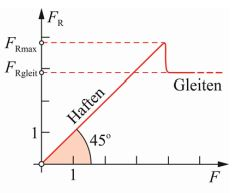
\includegraphics{bilder/reibungs}}
\end{minipage}


\subsubsection{Drehmoment}
\begin{minipage}{15cm}
Zwei entgegengesetzt gerichtete gleich grosse Kräfte mit 
parallelen, aber verschiedenen Wirkungslinien bilden ein 
Kräftepaar. Dies ergibt eine DREHWIRKUNG.
Eine drehende Wirkung lässt sich mit einem Kräftepaar oder, 
bezüglich eines Bezugspunktes, mit einer Einzelkraft erzielen.
Das Drehmoment eines Kräftepaars ist das Produkt des Betrags der Kraft und des Abstands der Wirkungslinien. \\
$M = a \cdot F$ , a ist der Abstand zum Drehpunkt \\
Drehmoment als Vektor im Raum: $\overrightarrow{M} = \overrightarrow{r} \times \overrightarrow{F} = F \cdot r \cdot \sin(\alpha)$ \\
 $\overrightarrow{M}$ steht im rechten Winkel auf der Ebene $\overrightarrow{r},  \overrightarrow{F}$ \\
Der Drehsinn ist in Gegenuhrzeigersinn. \\
\textbf{Tipp:} Der Bezugspunkt zu einem Drehmoment kann beliebig gewählt werden. Besonders geeignet sind Bezugspunkte, wo andere Kräfte Null ergeben!.  
\end{minipage}
\begin{minipage}{4cm}
\adjustbox{width=3cm}{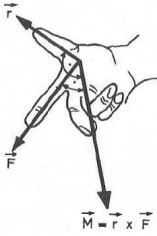
\includegraphics{bilder/drehmoment_2}}
\end{minipage}

\subsubsection{Schwerpunkt}
Der Schwerpunkt S eines Körpers ist der Punkt, in dem der unter der Wirkung der Schwerkraft stehende Körper unterstützt oder aufgehängt werden muss, damit er im Gleichgewicht ist. Der ausgedehnte Körper kann im Bezug auf die Schwerkraft durch einen Massenpunkt ersetzt werden. Eine Kraft auf den Schwerpunkt eines Körpers erzeugt kein Drehmoment (Abstand zum Drehpunkt ist Null)! \\
$ x_s = \frac{\Sigma_{i} x_{i} \cdot m_{i}}{\Sigma_{i} m_{i}}$
$ y_s = \frac{\Sigma_{i} y_{i} \cdot m_{i}}{\Sigma_{i} m_{i}}$
$ z_s = \frac{\Sigma_{i} z_{i} \cdot m_{i}}{\Sigma_{i} m_{i}}$ \\
Schwerpunkt eines Halbkreises: $x = 0,s \; y = \frac{4r}{3\pi}$ \\


\subsection{Deformierbare Körper}
- Elastisches Verhalten: Metalle, Keramik \\
- Plastisches  Verhalten: Plastilin, Knetmasse, Kunststoffe $\overrightarrow{}$ Mikroskopisches Modell mit Versetzung \\
- Moderne Materialien

\begin{multicols}{2}
\subsubsection{Spannung}
Die Kraft F kann in eine zur Fläche A senkrechte Konstante $F_{\perp}$ und eine zur Fläche parallele Konstante $F_{||}$ zerlegt werden.  \\
$\omega = \frac{F_{\perp}}{A} \; \; \tau = \frac{F_{||}}{A}$

\subsubsection{Dehnung / Längenkontraktion}
 Längenänderung $\Delta l:  \sim F / l / \frac{1}{A}$ \\
 Relative Verlängerung: $\frac{\Delta l}{l} = \varepsilon$ \\
Hookesche Gesetz: $ \varepsilon = \frac{1}{E} \cdot \sigma $ \\
Elastizitätsmodul E: \lbrack$ \frac{N}{m^2}$ \rbrack

\subsubsection{Kompression}

Volumenreduktion / Volumen: $\frac{\Delta V}{V} = - \kappa \Delta p$\\
Druckänderung: $\Delta$ p, \\
Kompressibilität $\kappa = \frac{3(1-2\mu)}{E}$


\subsubsection{Querkontraktion / Querdehnung}
Bei einer Längsdehnung eines Stabes tritt auch eine Querkontraktion auf, d.h. der Stab wird dünner. \\
$ \varepsilon_{q} = \frac{\Delta d}{d}$ d ist die Dicke, $\Delta d$ die Änderung der Dicke des Stabes \\
$\varepsilon_{q} = -\mu \varepsilon $ \\
Possionzahl $\mu$ ist zw. 0.15 und 0.5. 

\subsubsection{Schraubenfeder}
$F = c \Delta l, \;$ \\
Federkonstante $c = \frac{Gr^4}{4nR^3}$ \\
r = Drahtradius, n = Anz. Windungen, R = Windungsradius

\subsubsection{Schubbeanspruchung}
%\adjustbox{width=4.5cm}{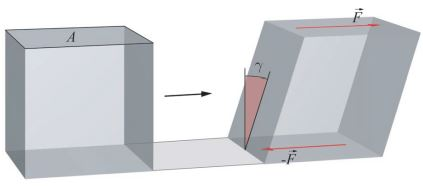
\includegraphics{bilder/schubbeanspruchung}}
$\gamma = \frac{1}{G}\tau$ \\
Schub-/Gleit-/Torsionsmodul G: $\frac{E}{2(1+\mu)} \lbrack \frac{N}{m^2} \rbrack$
\end{multicols}

\begin{multicols}{3}
\textbf{Torsionsfeder} \\
$M = c* \cdot \varphi$ \\
$c = \frac{\varphi G r^4}{2l} $
\columnbreak
\\
\textbf{Balken-Biegung} \\
$z = \frac{4l^3}{Ebh^3}F$ \\
b = Balkenbreite \\
\columnbreak
\\
\textbf{Skalierungsgesetz} \\
$z = \frac{5 \rho g l^4}{32Eh^2}$ \\
h = Höhe des Querschnitts
\end{multicols}


